\documentclass[border=2pt]{standalone}
\input{glyphtounicode}\pdfgentounicode=1
\usepackage{amsmath,amssymb}
\usepackage{newtxtext}
\usepackage{tikz}
\usetikzlibrary{arrows.meta,positioning,calc}
\definecolor{bbedge}{HTML}{5C82A6}\definecolor{bbfill}{HTML}{EAF1F7}
\definecolor{gtedge}{HTML}{C98A2E}\definecolor{gtfill}{HTML}{FBF1DF}
\definecolor{pbedge}{HTML}{8E5473}\definecolor{pbfill}{HTML}{F5ECF1}
\definecolor{outedge}{HTML}{5E8C61}\definecolor{outfill}{HTML}{EAF3EA}
\begin{document}
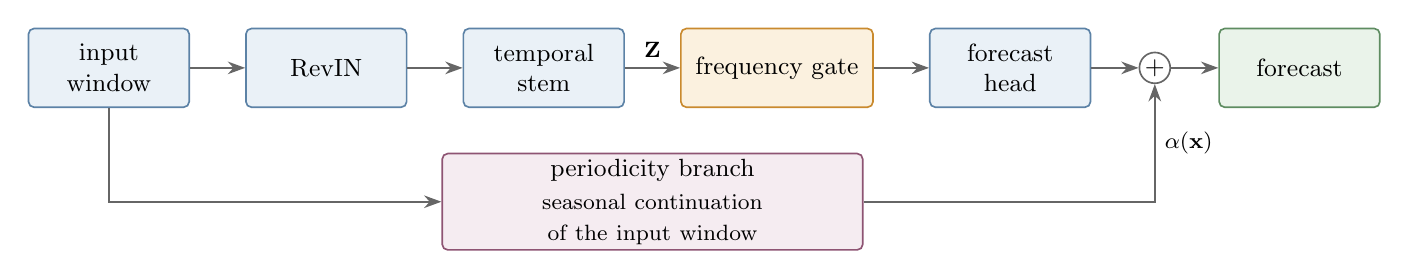
\begin{tikzpicture}[
  font=\small,
  >={Stealth[length=2.2mm,width=1.6mm]},
  box/.style={rectangle, rounded corners=2pt, line width=0.6pt, align=center,
              minimum height=10mm, text width=19mm, inner sep=2pt},
  bb/.style={box, draw=bbedge, fill=bbfill},
  arr/.style={->, line width=0.6pt, draw=black!60}
]
\node[bb] (in) {input\\window};
\node[bb, right=7mm of in] (rev) {RevIN};
\node[bb, right=7mm of rev] (stem) {temporal\\stem};
\node[box, draw=gtedge, fill=gtfill, right=7mm of stem, text width=23mm] (gate) {frequency gate};
\node[bb, right=7mm of gate] (head) {forecast\\head};
\node[circle, draw=black!60, line width=0.6pt, inner sep=0.6pt, right=6mm of head] (plus) {$+$};
\node[box, draw=outedge, fill=outfill, right=6mm of plus] (out) {forecast};
\node[box, draw=pbedge, fill=pbfill, text width=52mm, minimum height=11mm]
     (per) at ($(stem.east)!0.5!(gate.west) + (0,-17mm)$)
     {periodicity branch\\[1pt]{\footnotesize seasonal continuation of the input window}};
\draw[arr] (in) -- (rev);
\draw[arr] (rev) -- (stem);
\draw[arr] (stem) -- node[above, font=\footnotesize] {$\mathbf{Z}$} (gate);
\draw[arr] (gate) -- (head);
\draw[arr] (head) -- (plus);
\draw[arr] (plus) -- (out);
\draw[arr] (in.south) |- (per.west);
\draw[arr] (per.east) -| node[pos=0.75, right, font=\footnotesize] {$\alpha(\mathbf{x})$} (plus.south);
\end{tikzpicture}
\end{document}
